%**************************************************************************************
% License:
% CC BY-NC-SA 4.0 (http://creativecommons.org/licenses/by-nc-sa/4.0/)
%**************************************************************************************

\documentclass[notes]{beamer}

\mode<presentation> {

\usetheme{Madrid}

% Burnt orange
\definecolor{burntorange}{rgb}{0.8, 0.33, 0.0}
\colorlet{beamer@blendedblue}{burntorange}
% Pale yellow
\definecolor{paleyellow}{rgb}{1.0, 1.0, 0.953}
\setbeamercolor{background canvas}{bg=paleyellow}
% Secondary and tertiary palett
\setbeamercolor*{palette secondary}{use=structure,fg=white,bg=burntorange!80!black}
\setbeamercolor*{palette tertiary}{use=structure,fg=white,bg=burntorange!60!black}

% To remove the footer line in all slides uncomment this line
%\setbeamertemplate{footline}
% To replace the footer line in all slides with a simple slide count uncomment this line
%\setbeamertemplate{footline}[page number]

% To remove the navigation symbols from the bottom of all slides uncomment this line
%\setbeamertemplate{navigation symbols}{}
}

\usepackage{amsmath}
\usepackage{bm}
\usepackage{breqn}
\usepackage{fontawesome}
\usepackage{graphicx} % for figures
\usepackage{subcaption} % for subplots 
\usepackage[labelsep=space,tableposition=top]{caption}
\renewcommand{\figurename}{Fig.} 
\usepackage{cleveref}
\usepackage{caption,subcaption}% http://ctan.org/pkg/{caption,subcaption}
\usepackage{booktabs} % Allows the use of \toprule, \midrule and \bottomrule in tables
\usepackage{multirow}
\usepackage{xcolor}
\usepackage{empheq}
\usepackage[most]{tcolorbox}
\usepackage{listings}% http://ctan.org/pkg/listings
\lstset{basicstyle=\ttfamily,breaklines=true}
\usepackage{siunitx}
\usepackage{verbatim}

% To print 2 slides on a page
%\usepackage{handoutWithNotes}
%\pgfpagesuselayout{2 on 1}[border shrink=2mm]
%----------------------------------------------------------------------------------------
%	TITLE PAGE
%----------------------------------------------------------------------------------------
% The short title appears at the bottom of every slide, the full title is only on the title page
\title[CE 311K: Control flow]{CE 311K: Control flow - Branching and Iterations} 
\author{Krishna Kumar} % name
\institute[UT Austin] % institution 
{
University of Texas at Austin \\
\medskip
\href{mailto:krishnak@utexas.edu}{krishnak@utexas.edu} % email address
}
\date{\today} % Date, can be changed to a custom date

\begin{document}

\begin{frame}
\titlepage % title page as the first slide
\end{frame}

\newif\ifshowtoc
\showtoctrue% toggles to show the toc

\AtBeginSection{%
	\ifshowtoc
	\begin{frame}
		\tableofcontents[currentsection, subsectionstyle=show/show/hide]
	\end{frame}
	\fi
}

%----------------------------------------------------------------------------------------
% slides
%----------------------------------------------------------------------------------------
%------------------------------------------------

%------------------------------------------------
\section{Numerical solution of a sliding block}
\begin{frame}
	\frametitle{What is the optimal angle to pull the statue?}
	\begin{figure}[ht]
		\centering
		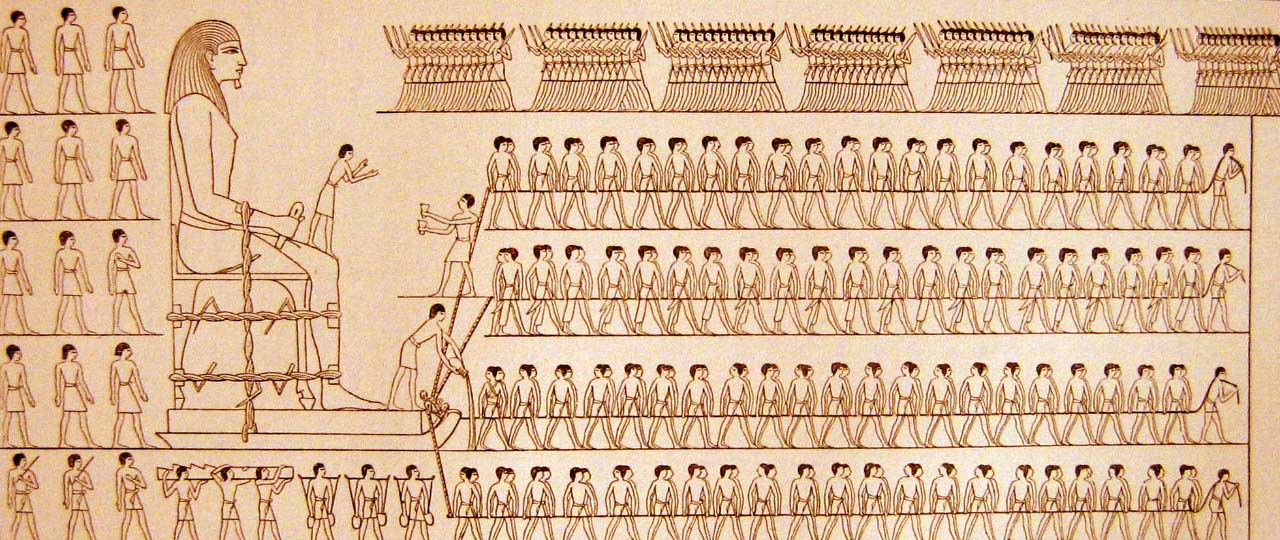
\includegraphics[width=\textwidth]{figs/egypt-pyramid.jpg}
		\caption*{A wall painting from the tomb of Djehutihotep (credit: martinhumanities.com)}
	\end{figure}
\end{frame}

%------------------------------------------------
\begin{frame}
	\frametitle{Numerical solution of a sliding block: Approximation}
	\begin{figure}[ht]
		\centering
		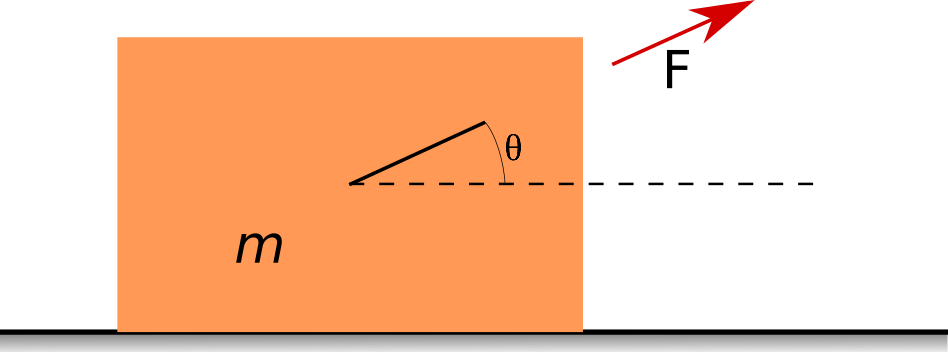
\includegraphics[width=0.85\textwidth]{figs/sliding-block.png}
		\caption*{What is the optimal angle to pull the block applying the least amount of force?}
	\end{figure}
\end{frame}


%------------------------------------------------
\begin{frame}
	\frametitle{Numerical solution of a sliding block: Forces}
	\mode<beamer>{		
		\begin{figure}[ht]
			\centering
			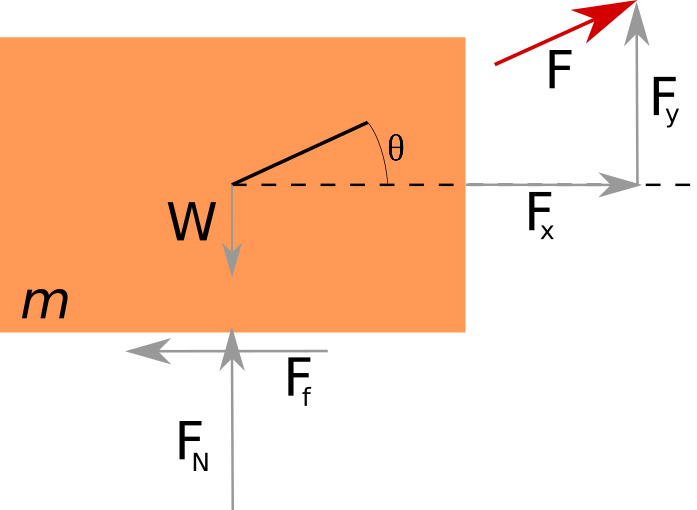
\includegraphics[width=0.85\textwidth]{figs/block-forces.png}
		\end{figure}
	}
	\mode<handout>{
		\begin{figure}[ht]
			\centering
			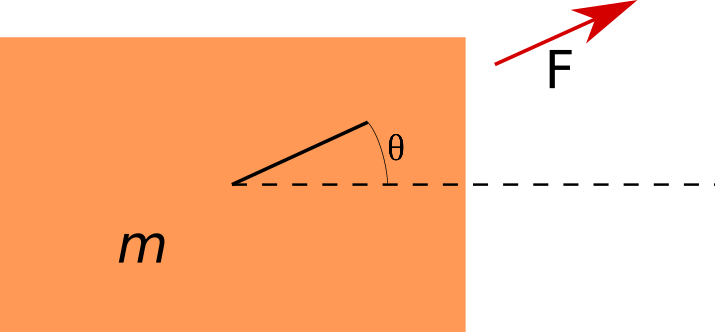
\includegraphics[width=0.85\textwidth]{figs/block-noforces.png}
		\end{figure}
	}
\end{frame}


%------------------------------------------------
\begin{frame}
	\frametitle{Numerical solution of a sliding block: Forces}
	\begin{minipage}[t]{0.7\linewidth}
		\mode<beamer>{		
			\begin{align*}
			& F_x = F \cos \theta \quad \& \quad F_y = F \sin \theta\\
			& F_f = \mu \cdot F_N = \mu \cdot W - \mu F_y = \mu m g - \mu F \sin \theta \\
			& \text{Vertical forces} \sum F_{vert} \uparrow: F_y + F_N - W = 0 \\
			& F_N = \mu m g - F \sin \theta \\
			& \text{Horizontal forces} \sum F_{hor} \rightarrow: F_x + F_f = 0 \\ 
			& F \cos \theta - \mu m g + \mu F \sin \theta = 0 \\
			\end{align*}
		}
		\mode<handout>{
			\vspace{4cm}
		}
	\end{minipage}%
	\hfill%
	\begin{minipage}[t]{0.29\linewidth}
		\begin{figure}[ht]
			\centering
			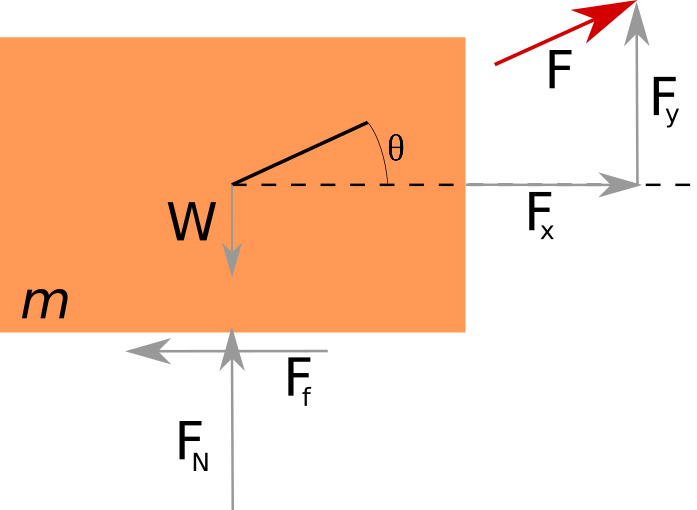
\includegraphics[width=\textwidth]{figs/block-forces.png}
		\end{figure}
	\end{minipage}%
	
	\begin{empheq}[box=\tcbhighmath]{equation*}
	F = \frac{\mu \cdot m g}{(\cos \theta + \mu \sin \theta)}
	\end{empheq}
\end{frame}

%------------------------------------------------
\begin{frame}
	\frametitle{Numerical solution of a sliding block: Compute force}
	\begin{itemize}
		\item Given $W = 25 kN (\SI{2500}{kg})$, $\theta = 45^o$ and $\mu = 0.75$ ($35^o$):
		\mode<beamer>{	
			\begin{equation*}
			F = \frac{0.75 \times 25 }{\cos(45) + 0.75 \sin(45)} = \SI{15.15}{kN}.
			\end{equation*}
		}
		\mode<handout>{
			\vspace{2.5cm}
		}
		\item Given $W = 25 kN (\SI{2500}{kg})$ and $\mu = 0.75$, what's the optimum $\theta$?
	\end{itemize}
\end{frame}

%------------------------------------------------
\begin{frame}
	\frametitle{\faCommentsO Numerical solution of a sliding block: Optimal theta?}
	Given $W = \SI{25}{\kilo\newton} (\SI{2500}{\kilogram})$ and $\mu = 0.75$, what's the optimum $\theta$?
	\begin{figure}[ht]
		\centering
		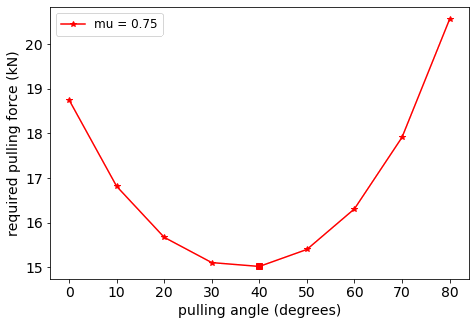
\includegraphics[width=0.8\textwidth]{figs/sliding-block-mu0p75-10.png}
	\end{figure}
\end{frame}

%------------------------------------------------
\begin{frame}[fragile]
	\frametitle{Lists}
	\begin{itemize}
		\item A list is a sequence of data. (mutable)
		\item An `array' in most other languages is a similar concept, but Python lists are more general than most arrays as they can hold a mixture of types. 
		\item A list is constructed using square brackets:
	\end{itemize}
	\begin{lstlisting}[language=Python]
>>> a = [0, 10, 20, 30, 40, 50, 60, 70, 80]
>>> print(a)
[0, 10, 20, 30, 40, 50, 60, 70, 80]
>>> type(a)
<class 'list'>
>>> len(a)
10
>>> a.append(90)
>>> print(a)
[0, 10, 20, 30, 40, 50, 60, 70, 80, 90]
	\end{lstlisting}
\end{frame}


%------------------------------------------------
\begin{frame}[fragile]
	\frametitle{Iterating through a list: for loops}
	
	Looping over each item in a list (or more generally a sequence) is called `iterating'. We iterate over the members of the lab group using the syntax:

	\begin{lstlisting}[language=Python]
for each item in list do
	print(item)
	\end{lstlisting}
	
	\begin{lstlisting}[language=Python]
for item in list:
	print(item)
	\end{lstlisting}
	
	\textcolor{red}{\faWarning ~Indentation matters in python!}
\end{frame}


%------------------------------------------------
\begin{frame}[fragile]
	\frametitle{range()}
	
	The \verb|range()| returns a sequence of numbers:
	
		\vspace{0.5cm}
		
		\verb|range(stop)|
		
		\vspace{0.5cm}
	
	\textit{stop:} Number of integers (whole numbers) to generate, starting from zero. eg. range(3) yields a sequence of [0, 1, 2].
	
	\vspace{0.5cm}
	
	\verb|range([start], stop[, step])|
	
	\begin{itemize}
		\item \textit{start}: Starting number of the sequence.
		\item \textit{stop}: Generate numbers up to, but not including this number.
		\item \textit{step}: Difference between each number in the sequence.
	\end{itemize}
	
\end{frame}

\note{
	Note that:
	\begin{itemize}
	\item All parameters must be integers.
	\item All parameters can be positive or negative.
	\item range() (and Python in general) is 0-index based, meaning list indexes start at 0, not 1		
	\end{itemize}
}


%------------------------------------------------
\begin{frame}
	\frametitle{Numerical solution of a sliding block: Optimal theta?}
	Given $W = \SI{25}{\kilo\newton} (\SI{2500}{\kilogram})$ and $\mu = 0.75$, what's the optimum $\theta$?
	\begin{figure}[ht]
		\centering
		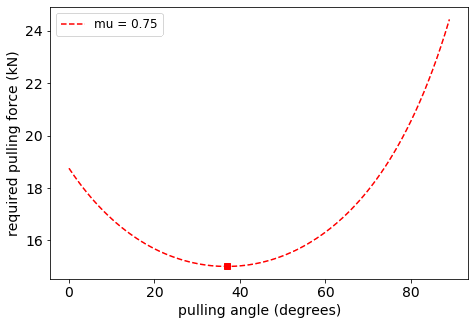
\includegraphics[width=0.75\textwidth]{figs/sliding-block-mu0p75.png}
		\caption*{\textcolor{red}{\faQuestionCircleO ~Identifying optimum requires conditional statements}}
	\end{figure}

\end{frame}

%------------------------------------------------
\begin{frame}[fragile]
	\frametitle{Comparison on int, float and strings}
	\texttt{i} and \texttt{j} are variable names and comparisons below evaluate to a Boolean
	\mode<beamer>{
		\begin{itemize}
			\item \texttt{i > j}
			\item \texttt{i >= j}
			\item \texttt{i < j}
			\item \texttt{i <=j}
			\item \texttt{i == j}: equality test, \texttt{True} if \texttt{i} is the same as \texttt{j}
			\item \texttt{i != j}: in equality test, \texttt{True} if \texttt{i} is not the same as \texttt{j}
		\end{itemize}
	}
	\mode<handout>{
		\vspace{5cm}
	}
\end{frame}

%------------------------------------------------
\begin{frame}[fragile]
	\frametitle{Logic operators on bools}
	\texttt{a} and \texttt{b} are variable names with Boolean values
	\mode<beamer>{
		\begin{itemize}
			\item \texttt{not a}: \texttt{True} if \texttt{a} is \texttt{False} \\
			\texttt{False} if \texttt{a} is \texttt{True}
			\item \texttt{a and b}: \texttt{True} if both are \texttt{True}.
			\item \texttt{a or b}: \texttt{True} if either or both are \texttt{True}.
		\end{itemize}
	}
	\mode<handout>{
		\vspace{3cm}
	}
	\begin{table}[!h]
		\begin{tabular}{llll}
			\toprule
			\texttt{A} & \texttt{B} & \texttt{A and B} & \texttt{A or B} \\
			\verb|True| & \verb|True| & \verb|True| & \verb|True| \\
			\verb|True| & \verb|False| & \verb|False| & \verb|True| \\
			\verb|False| & \verb|True| & \verb|False| & \verb|True| \\
			\verb|False| & \verb|False| & \verb|False| & \verb|False| \\
									
			\bottomrule
		\end{tabular}
	\end{table}
\end{frame}

%------------------------------------------------
\begin{frame}
	\frametitle{Designing a smart window: if condition}
	\begin{minipage}[t]{0.49\linewidth}
		\begin{figure}[ht]
			\centering
			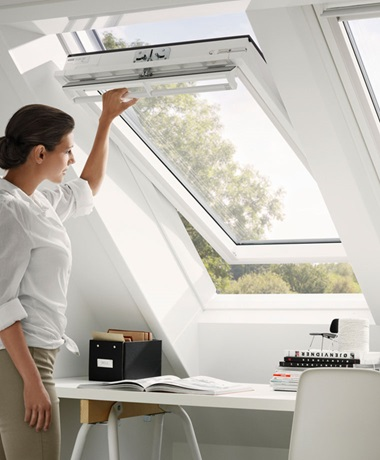
\includegraphics[width=0.62\textwidth]{figs/smart-window.jpg}
		\end{figure}
	\end{minipage}%
	\hfill%
	\begin{minipage}[t]{0.49\linewidth}
	\begin{itemize}
		\item An electric window opener, attached to a rain sensor and a temperature 
		gauge, might be controlled by the following program:
		\mode<beamer>{
		\item If raining: close window
		\item If too hot (80F): open window
		\item If too cold (66F): close window
		\item Otherwise: do nothing and leave window as it is
		}
	\end{itemize}
	\end{minipage}

\end{frame}

%------------------------------------------------
\begin{frame}[fragile]
	\frametitle{Designing a smart window: if condition}
	\begin{lstlisting}
# If raining, close the window
if raining:  
	close_window()

# If the temperature is over 80 F, open window
elif temperature > 80: # else if
	open_window()

# If the temperature is below 66 F, close window
elif temperature < 66:
	close_window()

# Otherwise, do nothing and leave window as it is
else:  
	continue
	\end{lstlisting}
\end{frame}

\note{
\texttt{<condition>} has a value \texttt{True} or \texttt{False}

evaluate \texttt{expressions} in that block if \texttt{<condition>} is True
}


%------------------------------------------------
\begin{frame}
	\frametitle{Numerical solution of a sliding block: Optimal theta?}
	Given $W = \SI{25}{\kilo\newton} (\SI{2500}{\kilogram})$ and $\mu = 0.75$, what's the optimum $\theta$?
	\begin{figure}[ht]
		\centering
		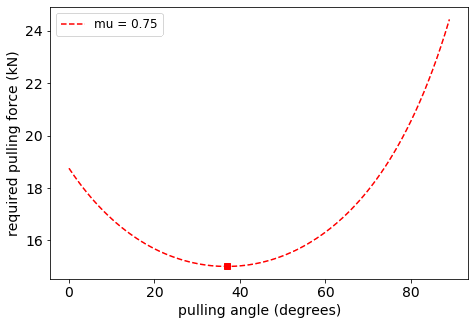
\includegraphics[width=0.75\textwidth]{figs/sliding-block-mu0p75.png}
		\caption*{\textcolor{blue}{Identify optimum with an if conditional statement}}
	\end{figure}
	
\end{frame}

%------------------------------------------------

\section{Bisection method}
%------------------------------------------------
\begin{frame}
	\frametitle{Calculate the optimum angle to pull for a given force}

	\begin{itemize}
		\item Given $F = \SI{17.5}{\kilo\newton} (\SI{1750}{kg})$, $W=\SI{25}{kN}$ and $\mu = 0.75$, what's $\theta$?
		\mode<beamer>{	
			\begin{align*}
			Try~\theta = 60^o:~ & F = \frac{0.75 \times 25 }{\cos(60) + 0.75 \sin(60)} = \SI{16.31}{kN}.\\
			Try~\theta = 70^o:~ & F = \frac{0.75 \times 25 }{\cos(70) + 0.75 \sin(70)} = \SI{17.91}{kN}.\\
			Try~\theta = 65^o:~ & F = \frac{0.75 \times 25 }{\cos(65) + 0.75 \sin(65)} = \SI{17.00}{kN}.\\
			Try~\theta = 67,5^o:~ & F = \frac{0.75 \times 25 }{\cos(67.5) + 0.75 \sin(67.5)} = \SI{17.43}{kN}.
			\end{align*}
			This is \textbf{bisection method!}
		}
		\mode<handout>{
			\vspace{4cm}
		}
	\end{itemize}
\end{frame}


%------------------------------------------------
\begin{frame}
	\frametitle{\faCommentsO ~What are the characteristics of a numerical solution?}
	\mode<beamer>{
		\begin{itemize}
			\item A numerical recipe is \textit{a sequence of simple steps}
			\item \textit{Flow of control} as each step is executed.
			\item Yields an \textit{approximate} numerical answer (a finite number) for the problem 
			\item These solutions can be very accurate
			\item Most answers are determined in an iterative approach (numerical method: mathematical / computer-aided technique) until a desired minimum/acceptable accuracy is obtained
			\item Typically, a finite set of iterations (steps) are used in the numerical method to obtain a solution. A means of determining \textit{when to stop}.
		\end{itemize}
	}
	\mode<handout>{
		\vspace{5cm}
	}
\end{frame}

%------------------------------------------------
\begin{frame}
	\frametitle{Numerical solution of a sliding block: Friction angles}	
	\begin{figure}[ht]
		\centering
		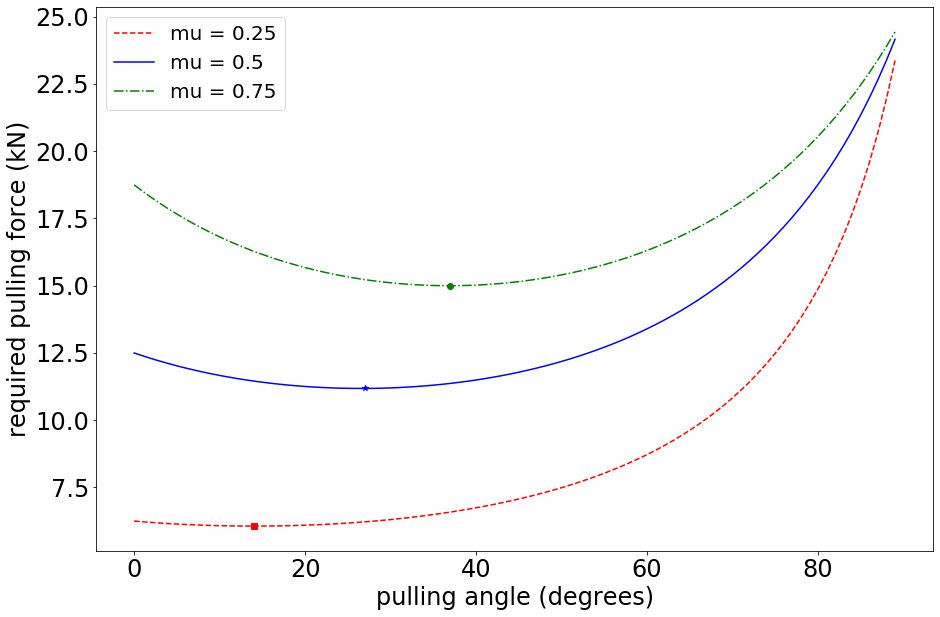
\includegraphics[width=0.85\textwidth]{figs/sliding-block-force-frictions.png}
	\end{figure}
\end{frame}

\end{document}